\subsubsection{Giới thiệu bộ dữ liệu}
    \paragraph{Nguồn dữ liệu}
    \leavevmode
    
    Bộ dữ liệu được thu thập bởi Martins và cộng sự \cite{martins2021early}, hỗ trợ bởi chương trình SATDAP - Capacitação da Administração Pública POCI-05-5762-FSE-000191, Bồ Đào Nha.

    \paragraph{Mô tả dữ liệu}
    \leavevmode
    
    Đây là bộ dữ liệu thu thập từ nhiều cơ sở giáo dục đại học hoặc tương đương, từ các ngành nông học, thiết kế, giáo dục, điều dưỡng, báo chí, quản lý, dịch vụ xã hội và công nghệ. Mỗi dòng dữ liệu bao gồm các thông tin yếu tố kinh tế xã hội tại thời điểm vào thời điểm sinh viên nhập học, các thông tin về cá nhân sinh viên, kèm kết quả học tập của sinh viên vào cuối học kỳ 1 và học kỳ 2 (hai học kỳ đầu tiên). Bộ dữ liệu bị thiếu dữ liệu ở bất kỳ cột nào.

    Ví dụ một phần dữ liệu:

    \begin{table}[htbp]
    \centering
    \caption{Một phần bảng dữ liệu student dropout}
    \label{tab:stat-dropout-exp}
    \begin{tabular}{|p{2cm}|p{2cm}|p{2.5cm}|p{2.5cm}|p{2cm}|}
        \hline
        Tuition fees up to date & Scholarship holder & Curricular units 1st sem (approved) & Curricular units 1st sem (grade) & ... \\
        \midrule
        1 & 0 & 0 & 0.000000 & ...\\
        \hline
        0 & 0 & 6 & 14.000000 & ...\\
        \hline
        0 & 0 & 0 & 0.000000 & ...\\
        \hline
        1 & 0 & 6 & 13.428571 & ...\\
        \hline
        1 & 0 & 5 & 12.333333 & ...\\
        \hline
        1 & 0 & 5 & 11.857143 & ...\\
        \hline
        ... & ... & ... & ... & ...\\
        \hline
    \end{tabular}
    \end{table}

    \FloatBarrier

    Bộ dữ liệu có 4424 dòng, bao gồm 37 cột như sau:
    \begin{itemize}
        \item Kiểu dữ liệu: \textbf{Quantitative} 

        \begin{enumerate}
            \item \textbf{Marital Status}: Tình trạng hôn nhân

            Các giá trị:

            \begin{itemize}
              \item \textbf{1}: Độc thân
              \item \textbf{2}: Kết hôn
              \item \textbf{3}: Góa chồng/vợ
              \item \textbf{4}: Ly dị
              \item \textbf{5}: Sống chung (không pháp lý)
              \item \textbf{6}: Ly thân
            \end{itemize}

            \item \textbf{Application mode}: Trạng thái xét tuyển

            Các giá trị:
            
            \begin{itemize}
              \item \textbf{1}: Giai đoạn 1 – Diện tuyển sinh chung
              \item \textbf{2}: Theo Quy định số 612/93
              \item \textbf{5}: Giai đoạn 1 – diện đặc biệt (Quần đảo Azores)
              \item \textbf{7}: Người đã có văn bằng giáo dục đại học khác
              \item \textbf{10}: Theo Quy định số 854-B/99
              \item \textbf{15}: Sinh viên quốc tế (bậc cử nhân)
              \item \textbf{16}: Giai đoạn 1 – diện đặc biệt (Quần đảo Madeira)
              \item \textbf{17}: Giai đoạn 2 – diện tuyển sinh chung
              \item \textbf{18}: Giai đoạn 3 – diện tuyển sinh chung
              \item \textbf{26}: Theo Quy định số 533-A/99, mục b2 (Chương trình khác)
              \item \textbf{27}: Theo Quy định số 533-A/99, mục b3 (Trường khác)
              \item \textbf{39}: Trên 23 tuổi
              \item \textbf{42}: Chuyển trường
              \item \textbf{43}: Chuyển ngành học
              \item \textbf{44}: Người có văn bằng chuyên môn công nghệ
              \item \textbf{51}: Chuyển trường/ngành học
              \item \textbf{53}: Người có văn bằng chương trình ngắn hạn
              \item \textbf{57}: Chuyển trường/ngành học (Sinh viên quốc tế)
            \end{itemize}

            \item \textbf{Course}: Mã ngành

            Các giá trị:

            \begin{itemize}
              \item \textbf{33}: Công nghệ sản xuất nhiên liệu sinh học
              \item \textbf{171}: Thiết kế hoạt hình và đa phương tiện
              \item \textbf{8014}: Công tác xã hội (hệ học buổi tối)
              \item \textbf{9003}: Nông học
              \item \textbf{9070}: Thiết kế truyền thông
              \item \textbf{9085}: Điều dưỡng thú y
              \item \textbf{9119}: Kỹ thuật tin học
              \item \textbf{9130}: Kỹ thuật nuôi ngựa
              \item \textbf{9147}: Quản trị
              \item \textbf{9238}: Công tác xã hội
              \item \textbf{9254}: Du lịch
              \item \textbf{9500}: Điều dưỡng
              \item \textbf{9556}: Vệ sinh răng miệng
              \item \textbf{9670}: Quản trị quảng cáo và tiếp thị
              \item \textbf{9773}: Báo chí và truyền thông
              \item \textbf{9853}: Giáo dục tiểu học
              \item \textbf{9991}: Quản trị (hệ học buổi tối)
            \end{itemize}

            \item \textbf{Daytime/evening attendance}: Buổi học
            
            Các giá trị:
            \begin{itemize}
                \item \textbf{0}: Tối
                \item \textbf{1}: Sáng
            \end{itemize}

            \item \textbf{Previous qualification}: Trình độ khi xét tuyển

            Các giá trị:
            \begin{itemize}
              \item \textbf{1}: Giáo dục trung học phổ thông
              \item \textbf{2}: Giáo dục đại học –  bằng cử nhân
              \item \textbf{3}: Giáo dục đại học – bằng không rõ
              \item \textbf{4}: Giáo dục đại học – bằng thạc sĩ
              \item \textbf{5}: Giáo dục đại học – bằng tiến sĩ
              \item \textbf{6}: Đang theo học đại học
              \item \textbf{9}: Chưa hoàn thành Lớp 12
              \item \textbf{10}: Chưa hoàn thành Lớp 11
              \item \textbf{12}: Khác – trình độ tương đương lớp 11
              \item \textbf{14}: Lớp 10
              \item \textbf{15}: Chưa hoàn thành Lớp 10
              \item \textbf{19}: Lớp 9/10/11 hoặc tương đương
              \item \textbf{38}: Lớp 6/7/8 hoặc tương đương
              \item \textbf{39}: Đã học khóa chuyên môn công nghệ
              \item \textbf{40}: Trình độ cử nhân (EU)
              \item \textbf{42}: Đã học khóa kỹ thuật cao đẳng chuyên nghiệp
              \item \textbf{43}: Trình độ thạc sĩ (EU)
            \end{itemize}

            \item \textbf{Nacionality}: Quốc tịch

            Các giá trị:
            \begin{itemize}
              \item \textbf{1}: Bồ Đào Nha
              \item \textbf{2}: Đức
              \item \textbf{6}: Tây Ban Nha
              \item \textbf{11}: Ý
              \item \textbf{13}: Hà Lan
              \item \textbf{14}: Anh
              \item \textbf{17}: Litva
              \item \textbf{21}: Angola
              \item \textbf{22}: Cabo Verde
              \item \textbf{24}: Guinée-Bissau
              \item \textbf{25}: Mozambique
              \item \textbf{26}: Santomean
              \item \textbf{32}: Thổ Nhĩ Kỳ
              \item \textbf{41}: Brazil
              \item \textbf{62}: Romania
              \item \textbf{100}: Moldova
              \item \textbf{101}: Mexico
              \item \textbf{103}: Ukraina
              \item \textbf{105}: Nga
              \item \textbf{108}: Cuba
              \item \textbf{109}: Colombia
            \end{itemize}

            \item \hypertarget{line:1-mom-qua}{\textbf{Mother's qualification}}: Trình độ học vấn mẹ

            Các giá trị: 
            \begin{itemize}
              \item \textbf{1}: Trung học phổ thông – lớp 12 hoặc tương đương
              \item \textbf{2}: Giáo dục đại học – Cử nhân
              \item \textbf{3}: Giáo dục đại học – Bằng tốt nghiệp đại học
              \item \textbf{4}: Giáo dục đại học – Thạc sĩ
              \item \textbf{5}: Giáo dục đại học – Tiến sĩ
              \item \textbf{6}: Đang theo học giáo dục đại học
              \item \textbf{9}: Lớp 12 – chưa hoàn thành
              \item \textbf{10}: Lớp 11 – chưa hoàn thành
              \item \textbf{11}: Lớp 7 (theo hệ thống cũ)
              \item \textbf{12}: Khác – trình độ tương đương lớp 11
              \item \textbf{13}: Năm 2 bổ túc trung học phổ thông
              \item \textbf{14}: Lớp 10
              \item \textbf{18}: Đã học khóa thương mại tổng quát
              \item \textbf{19}: Lớp 9/10/11 hoặc tương đương
              \item \textbf{20}: Đã học khóa bổ túc trung học phổ thông
              \item \textbf{22}: Đã học khóa kỹ thuật – nghề nghiệp
              \item \textbf{25}: Khóa bổ túc trung học phổ thông - chưa hoàn thành
              \item \textbf{26}: Lớp 7
              \item \textbf{27}: Lớp 6/7/8 hoặc tương đương
              \item \textbf{29}: Lớp 9 – chưa hoàn thành
              \item \textbf{30}: Lớp 8
              \item \textbf{31}: Đã học khóa Quản trị và Thương mại
              \item \textbf{33}: Đã học khóa bổ túc Kế toán và Quản trị
              \item \textbf{34}: Không rõ
              \item \textbf{35}: Không biết đọc hoặc viết
              \item \textbf{36}: Biết đọc nhưng chưa học đến lớp 4
              \item \textbf{37}: Lớp 4/5 hoặc tương đương
              \item \textbf{38}: Lớp 6/7/8 hoặc tương đương
              \item \textbf{39}: Đã học khóa chuyên môn công nghệ
              \item \textbf{40}: Trình độ cử nhân (chương trình chuẩn EU)
              \item \textbf{41}: Đã học khóa chuyên ngành cao học
              \item \textbf{42}: Đã học khóa cao đẳng kỹ thuật chuyên nghiệp
              \item \textbf{43}: Thạc sĩ (chương trình chuẩn EU)
              \item \textbf{44}: Tiến sĩ (chương trình chuẩn EU)
            \end{itemize}

            \item \textbf{Father's qualification}: Trình độ học vấn cha
            
            Các giá trị: (tương tự \hyperlink{line:1-mom-qua}{\textit{\textbf{Mother's qualification}}})

            \item \hypertarget{line:1-mom-job}{\textbf{Mother's occupation}}: Nghề nghiệp mẹ

            Các giá trị:
            \begin{itemize}
              \item \textbf{0}: Đang trong quá trình học tập
              \item \textbf{1}: Đại biểu cơ quan lập pháp, cơ quan hành pháp, giám đốc hoặc quản lý cấp cao
              \item \textbf{2}: Chuyên gia trong các lĩnh vực trí tuệ và khoa học
              \item \textbf{3}: Kỹ thuật viên và chuyên viên trình độ trung cấp
              \item \textbf{4}: Nhân viên hành chính
              \item \textbf{5}: Nhân viên dịch vụ cá nhân, an ninh và bán hàng
              \item \textbf{6}: Nông dân và lao động lành nghề trong nông nghiệp, ngư nghiệp, lâm nghiệp
              \item \textbf{7}: Lao động lành nghề trong công nghiệp, xây dựng và thủ công
              \item \textbf{8}: Công nhân lắp đặt, vận hành máy móc và lắp ráp
              \item \textbf{9}: Lao động phổ thông
              \item \textbf{10}: Quân nhân
              \item \textbf{90}: Khác
              \item \textbf{99}: Không rõ
              \item \textbf{101}: Sĩ quan quân đội
              \item \textbf{102}: Hạ sĩ quan quân đội
              \item \textbf{103}: Nhân sự  lực lượng vũ trang
              \item \textbf{112}: Giám đốc dịch vụ hành chính và thương mại
              \item \textbf{114}: Giám đốc khách sạn, ăn uống, thương mại và các dịch vụ tương tự khác
              \item \textbf{121}: Chuyên gia khoa học tự nhiên, toán học, kỹ thuật và các lĩnh vực liên quan
              \item \textbf{122}: Nhân viên y tế
              \item \textbf{123}: Giáo viên
              \item \textbf{124}: Chuyên gia tài chính, kế toán, tổ chức hành chính, quan hệ công – thương
              \item \textbf{125}: Chuyên gia công nghệ thông tin và truyền thông
              \item \textbf{131}: Kỹ thuật viên trung cấp trong khoa học và kỹ thuật
              \item \textbf{132}: Kỹ thuật viên trung cấp trong lĩnh vực y tế
              \item \textbf{134}: Kỹ thuật viên trung cấp trong lĩnh vực pháp luật, xã hội, thể thao, văn hóa
              \item \textbf{135}: Kỹ thuật viên công nghệ thông tin và truyền thông
              \item \textbf{141}: Nhân viên văn phòng, thư ký, và nhân viên xử lý dữ liệu
              \item \textbf{143}: Nhân viên dữ liệu, kế toán, thống kê, tài chính và lưu trữ
              \item \textbf{144}: Nhân viên hỗ trợ hành chính
              \item \textbf{151}: Giúp việc
              \item \textbf{152}: Nhân viên bán hàng
              \item \textbf{153}: Nhân viên chăm sóc cá nhân và tương tự
              \item \textbf{154}: Nhân viên bảo vệ và dịch vụ an ninh
              \item \textbf{161}: Nông dân định hướng thị trường và lao động lành nghề trong nông nghiệp, chăn nuôi
              \item \textbf{163}: Nông dân tự cung tự cấp, người chăn nuôi, ngư dân, thợ săn và hái lượm
              \item \textbf{171}: Lao động lành nghề trong xây dựng (trừ thợ điện)
              \item \textbf{172}: Lao động lành nghề trong luyện kim, gia công kim loại và tương tự
              \item \textbf{173}: Lao động lành nghề trong in ấn, sản xuất thiết bị chính xác, kim hoàn, thủ công
              \item \textbf{174}: Lao động lành nghề trong điện và điện tử
              \item \textbf{175}: Công nhân chế biến thực phẩm, gỗ, may mặc và các ngành thủ công khác
              \item \textbf{181}: Công nhân vận hành thiết bị và máy móc cố định
              \item \textbf{182}: Công nhân dây chuyền
              \item \textbf{183}: Lái xe/Công nhân vận hành thiết bị di động
              \item \textbf{191}: Nhân viên vệ sinh
              \item \textbf{192}: Lao động phổ thông trong nông nghiệp, chăn nuôi, thủy sản và lâm nghiệp
              \item \textbf{193}: Lao động phổ thông trong khai khoáng, xây dựng, sản xuất và vận tải
              \item \textbf{194}: Nhân viên phụ bếp
              \item \textbf{195}: Bán hàng rong hoặc cung cấp dịch vụ đường phố (trừ liên quan đến thực phẩm)
            \end{itemize}

            \item \textbf{Father's occupation}: Nghề nghiệp cha
    
            Các giá trị: (tương tự \hyperlink{line:1-mom-job}{\textit{\textbf{Mother's occupation}}})
    
            \item \textbf{Displaced}: Người tị nạn
            
            Các giá trị:
            \begin{itemize}
                \item \textbf{0}: Không
                \item \textbf{1}: Đúng
            \end{itemize}
    
             \item \textbf{Educational special needs}: Cần giáo dục đặc biệt
            
            Các giá trị:
            \begin{itemize}
                \item \textbf{0}: Không
                \item \textbf{1}: Có
            \end{itemize}
    
            \item \textbf{Debtor}: Mắc nợ
            
            Các giá trị:
            \begin{itemize}
                \item \textbf{0}: Không
                \item \textbf{1}: Có
            \end{itemize}
    
            \item \textbf{Tuition fees up to date}: Đóng học phí đầy đủ
            
            Các giá trị:
            \begin{itemize}
                \item \textbf{0}: Không
                \item \textbf{1}: Đúng
            \end{itemize}
    
            \item \textbf{Gender}: Giới tính
            
            Các giá trị:
            \begin{itemize}
                \item \textbf{0}: Nữ
                \item \textbf{1}: Nam
            \end{itemize}

            \item \textbf{Scholarship holder}: Học bổng
            
            Các giá trị:
            \begin{itemize}
                \item \textbf{0}: Không
                \item \textbf{1}: Có
            \end{itemize}

            \item \textbf{International}: Học sinh quốc tế
            
            Các giá trị:
            \begin{itemize}
                \item \textbf{0}: Không
                \item \textbf{1}: Đúng
            \end{itemize}

            \item \textbf{Target}: Tình trạng sinh viên
            
            Các giá trị:
            \begin{itemize}
                \item \textbf{Graduate}: Đã tốt nghiệp
                \item \textbf{Enrolled}: Đang học
                \item \textbf{Dropout}: Đã bỏ học
            \end{itemize}
            
        \end{enumerate}

        \item Kiểu dữ liệu: \textbf{Qualitative} 
        \begin{itemize}
            \item \textbf{Discrete}:
                \begin{enumerate}[resume]
                    \item \textbf{Application order}: Xét tuyển vào trường là nguyện vọng thứ mấy (0 - nguyện vọng 1, đếm lên)
    
                    \item \textbf{Age at enrollment}: Tuổi nhập học
    
                    \item \textbf{Curricular units 1st sem (credited)}: Số học phần được miễn học kỳ 1
                    
                    \item \textbf{Curricular units 1st sem (enrolled)}: Số học phần đăng ký học kỳ 1
                    
                    \item \textbf{Curricular units 1st sem (evaluations)}: Số học phần được đánh giá học kỳ 1
                    
                    \item \textbf{Curricular units 1st sem (approved)}: Số học phần qua môn trong học kỳ 1
                    
                    \item \textbf{Curricular units 1st sem (without evaluations)}: Số học phần không đánh giá học kỳ 1
                    
                    \item \textbf{Curricular units 2nd sem (credited)}: Số học phần được miễn học kỳ 2
                    
                    \item \textbf{Curricular units 2nd sem (enrolled)}: Số học phần đăng ký học kỳ 2
                    
                    \item \textbf{Curricular units 2nd sem (evaluations)}: Số học phần được đánh giá học kỳ 2
                    
                    \item \textbf{Curricular units 2nd sem (approved)}: Số học phần qua môn trong học kỳ 2
                    
                    \item \textbf{Curricular units 2nd sem (without evaluations)}: Số học phần không đánh giá học kỳ 2
                \end{enumerate}

            \item \textbf{Continuous}:
                \begin{enumerate}[resume]
                    \item \textbf{Previous qualification (grade)}: Điểm bằng cấp trước đó

                    \item \textbf{Admission grade}: Điểm đầu vào
                
                    \item \textbf{Curricular units 1st sem (grade)}: Điểm trung bình học kỳ 1 (trong khoảng 0-20\hypertarget{line:1-grade1}{*})

                    \item \textbf{Curricular units 2nd sem (grade)}: Điểm trung bình học kỳ 2 (trong khoảng 0-20)

                    \item \textbf{Unemployment rate}: Tỉ lệ thất nghiệp khi người đó nhập học

                    \item \textbf{Inflation rate}: Tỉ lệ lạm phát khi người đó nhập học
                    
                    \item \textbf{GDP}: GDP khi người đó nhập học
                    
                \end{enumerate}

            
        \end{itemize}
        
    \end{itemize}
    

\subsubsection{Các nghiên cứu liên quan}
Tác giả của bài báo \cite{2023} sử dụng các mô hình học máy (Machine Learning) để dự đoán tình trạng sinh viên tốt nghiệp đúng hạn. Nghiên cứu này nhằm lựa chọn mô hình học máy tối ưu để dự đoán tình trạng sinh viên tốt nghiệp đúng hạn, đồng thời xác định các thuộc tính thông tin có tác động mạnh đến khả năng tốt nghiệp đúng hạn hoặc quá hạn của sinh viên, từ đó đề xuất khuyến nghị giúp nhà trường nâng cao tỷ lệ tốt nghiệp. Để thực hiện mục tiêu này, bài báo sử dụng tập dữ liệu của 6.696 sinh viên chuyên ngành Ngân hàng thuộc Học viện Ngân hàng Hà Nội từ năm 2010 đến 2020. Dữ liệu đã được tiền xử lý bằng cách làm sạch, chuyển đổi, mã hóa, chia thành tập huấn luyện và kiểm tra theo tỷ lệ 80:20, và đặc biệt là áp dụng kỹ thuật SMOTE để xử lý tình trạng mất cân bằng dữ liệu (86,96\% "Đúng hạn" và 13,04\% "Quá hạn"). Nghiên cứu đã thử nghiệm 7 mô hình học máy: Logistic Regression (LR), K-Nearest Neighbors (KNN), Decision Tree (DT), Random Forest (RF), Support Vector Machine (SVM), XGBoost và CatBoost, và đánh giá hiệu suất của chúng dựa trên các chỉ số như Precision, Recall, Accuracy, và đặc biệt là F1 Score, cùng với kỹ thuật LIME để giải thích sự đóng góp của các thuộc tính. Kết quả nghiên cứu cho thấy Random Forest (RF) là mô hình tối ưu nhất, đạt độ chính xác 92\% và điểm F1 là 92\%, vượt trội so với các mô hình khác (XGBoost và CatBoost đạt 89\% F1, LR và SVM đạt 80\% F1).

Nghiên cứu tiếp theo này \cite{article_tab_1} tập trung vào việc dự đoán chất lượng không khí ở Jakarta, cụ thể là nồng độ PM2.5, nhằm phát triển một mô hình dự đoán chính xác và có khả năng giải thích được thông qua việc sử dụng khuôn khổ XGBoost-SHAP. Mục tiêu chính là không chỉ dự đoán nồng độ PM2.5 một cách đáng tin cậy mà còn cung cấp những hiểu biết sâu sắc về các đặc điểm ảnh hưởng đáng kể nhất đến các dự đoán đó, từ đó cung cấp thông tin thực tế cho cộng đồng và cơ sở dữ liệu cho các nhà hoạch định chính sách để xây dựng các chiến lược giảm thiểu ô nhiễm. Để đạt được điều này, nghiên cứu đã sử dụng dữ liệu thứ cấp về Chỉ số Tiêu chuẩn Ô nhiễm Không khí (ISPU) của tỉnh DKI Jakarta từ tháng 1 năm 2021 đến tháng 5 năm 2024, bao gồm 4774 điểm dữ liệu hàng ngày từ 5 trạm quan trắc. Dữ liệu này bao gồm các thuộc tính như PM10, PM2.5, SO2, CO, O3, NO2, giá trị "max" (giá trị cao nhất của các tham số được theo dõi), "critical" (tham số có giá trị ISPU cao nhất), và "category" (loại chất lượng không khí). Quá trình tiền xử lý dữ liệu bao gồm xử lý các giá trị thiếu (41 hàng thiếu trong cột "critical" được điền bằng mode, các giá trị '0' trong các cột số được xử lý bằng KNN Imputer với k=5), mã hóa các biến phân loại sử dụng Label Encoder, và xử lý dữ liệu ngoại lai bằng phương pháp Winsorizing. Mô hình học máy chính được áp dụng là XGBoost, được lựa chọn vì khả năng xử lý dữ liệu phức tạp và ngăn ngừa overfitting. Điều chỉnh siêu tham số (hyperparameter tuning) cho XGBoost được thực hiện bằng Grid Search với cơ chế kiểm định chéo 10 lần (10-fold cross-validation). Dữ liệu được chia thành tập huấn luyện và kiểm tra với ba tỷ lệ (90:10, 80:20, 70:30), và hiệu suất mô hình được đánh giá bằng MSE, RMSE, R2, và đặc biệt là MAPE (Mean Absolute Percentage Error), với MAPE dưới 10\% được coi là "chính xác". Kết quả cho thấy mô hình XGBoost đạt hiệu suất vượt trội, với MAPE thấp nhất là 4.44\% khi sử dụng tỷ lệ dữ liệu kiểm thử 10\%, giá trị này dưới 10\% cho thấy khả năng dự đoán chính xác. So với các nghiên cứu trước đây về dự đoán PM2.5, mô hình XGBoost này cho thấy hiệu suất tốt hơn so với Hybrid ARIMA-ANN (MAPE 13.6\%), LSTM (MAPE 8.07\%), và Ordinary Kriging (MAPE 19.5\%). Phân tích SHAP đã cung cấp những hiểu biết quan trọng, chỉ ra rằng đặc điểm "max" có ảnh hưởng lớn nhất đến dự đoán, tiếp theo là PM10 (có xu hướng làm tăng nồng độ PM2.5). Nhìn chung, nghiên cứu kết luận rằng mô hình XGBoost có thể được sử dụng hiệu quả để dự đoán nồng độ PM2.5 với độ chính xác cao và các phát hiện này đóng góp đáng kể vào việc hiểu các tương tác giữa các thông số chất lượng không khí, cung cấp cơ sở cho việc ra quyết định trong các nỗ lực giảm thiểu ô nhiễm không khí tại khu vực DKI Jakarta

\subsubsection{Phân tích dữ liệu}
    \paragraph{Thống kê dữ liệu}
    \leavevmode

    \hypertarget{line:stat-example}{\textbf{Tính các thông số thống kê:}}

    Lấy cột 'Curricular units 1st sem (grade)', ta thực hiện tính các thông số thống kê

    \begin{lstlisting}[language=Python]
        sem1_grade = df_raw['Curricular units 1st sem (grade)']
    \end{lstlisting}
    
    \begin{itemize}
        \item Mean:
            Áp dụng công thức \ref{eq:Mean}

\begin{lstlisting}[language=Python]
    mean_sem1_grade = sem1_grade.sum() / sem1_grade.count()
    
    -> 10.640821575154185
\end{lstlisting}

        \item Q1: Áp dụng công thức \ref{eq:percentile-position-2}
\begin{lstlisting}[language=Python]
    pos = 0.25 * (n + 1)
    k = int(np.floor(pos))
    d = pos - k
    
    if k <= 0:
        q1_sem1_grade = sem1_grade.iloc[0]
    else:
        lower = sem1_grade.iloc[k - 1]
        upper = sem1_grade.iloc[k]
        q1_sem1_grade = lower + d * (upper - lower)
    
    -> 11.0
\end{lstlisting}

        \item Median: Dữ liệu có n=4424, theo công thức \ref{eq:median_0}
\begin{lstlisting}[language=Python]
    median_sem1_grade = (
        sem1_grade.iloc[n//2 - 1] + sem1_grade.iloc[n//2]
    ) / 2
    
    -> 12.285714285714286
\end{lstlisting}
            
        \item Q3: Áp dụng công thức \ref{eq:percentile-position-2}
\begin{lstlisting}[language=Python]
    pos = 0.75 * (n + 1)
    k = int(np.floor(pos))
    d = pos - k
    
    if k >= n:
        q3_sem1_grade = sem1_grade.iloc[-1]
    else:
        lower = sem1_grade.iloc[k - 1]
        upper = sem1_grade.iloc[k]
        q3_sem1_grade = lower + d * (upper - lower)

    ->  13.4
\end{lstlisting}

        \item Mode: Áp dụng công thức \ref{eq:Mode}
\begin{lstlisting}[language=Python]
    counts = sem1_grade.value_counts()
    max_count = counts.max()
    modes = counts[counts == max_count].index.tolist()

    ->  0.0
\end{lstlisting}

        \item IQR: Từ Q3 và Q1 ta có \ref{eq:iqr} IQR = 13.4 - 11.0 = 2.4
            

        \item Variance: Áp dụng \ref{eq:population-variance}
\begin{lstlisting}[language=Python]
   squared_diffs = [(x - mean_sem1_grade) ** 2 for x in sem1_grade]

    var_sem1_grade = sum(squared_diffs) / n

    -> 23.455771808893843
\end{lstlisting}

         \item Standard Deviation: Áp dụng \ref{eq:population-sd}
\begin{lstlisting}[language=Python]
   sd_sem1_grade = math.sqrt(var_sem1_grade)

   ->  4.843115919415293
\end{lstlisting}

          \item Coefficient of Variation: Áp dụng \ref{eq:cv-population}
\begin{lstlisting}[language=Python]
   cv_sem1_grade = sd_sem1_grade / mean_sem1_grade

   -> 0.4551449232758249
\end{lstlisting}
        \end{itemize}

    Thực hiện tương tự, ta thu được bảng \ref{tab:stat-dropout} thể hiện các thông số thống kê trên một số đặc trưng của bộ dữ liệu.    
    
    \begin{table}[htbp]
    \centering
    \caption{ Thống kê dữ liệu một số đặc trưng dữ liệu sinh viên}
    \label{tab:stat-dropout}
    \begin{tabular}{|p{2cm}|p{2cm}|p{2cm}|p{2cm}|p{2cm}|p{2cm}|p{2cm}|}
        \hline
        Thông số & Application order & Age at enrollment & Curricular units 1st sem (approved) & Curricular units 1st sem (grade) & Curricular units 2nd sem (approved) & Curricular units 2nd sem (grade) \\
        \hline
        Mean & 1.7278 & 23.2651 & 4.7066 & 10.6408 & 4.4358 & 10.2302 \\
        Min & 0.0000 & 17.0000 & 0.0000 & 0.0000 & 0.0000 & 0.0000 \\
        Q1 & 1.0000 & 19.0000 & 3.0000 & 11.0000 & 2.0000 & 10.7500 \\
        Median & 1.0000 & 20.0000 & 5.0000 & 12.2857 & 5.0000 & 12.2000 \\
        Q3 & 2.0000 & 25.0000 & 6.0000 & 13.4000 & 6.0000 & 13.3333 \\
        Max & 9.0000 & 70.0000 & 26.0000 & 18.8750 & 20.0000 & 18.5714 \\
        Mode & 1.0000 & 18.0000 & 6.0000 & 0.0000 & 6.0000 & 0.0000 \\
        Variance & 1.7261 & 57.5749 & 9.5743 & 23.4611 & 9.0888 & 27.1525 \\
        SD & 1.3138 & 7.5878 & 3.0942 & 4.8437 & 3.0148 & 5.2108 \\
        CV & 0.7604 & 0.3261 & 0.6574 & 0.4552 & 0.6796 & 0.5094 \\
        IQR & 1.0000 & 6.0000 & 3.0000 & 2.4000 & 4.0000 & 2.5833 \\
        \hline
    \end{tabular}
    \end{table}

    Từ đây, ta có thể rút ra một số nhận xét:

    \begin{itemize}
        \item Application order: Có trung vị 1, trung bình $\approx$ 1.73 và mode 1, cho thấy đa số sinh viên đậu vào trường ở nguyện vọng 2 của họ. Cho thấy đa số sinh viên thường chọn nguyện vọng 1 là mục tiêu cao hơn, và nguyện vọng 2 là vị trí an toàn cho khả năng của họ.

        \item Age at enrollment: Mode = 18 cho thấy tuổi sinh viên nhập học nhiều nhất là ngay vừa tốt nghiệp xong trung học. Trung bình 23.265, trung vị 20 cho thấy phân phối tuổi lệch về phải. 

        \item Curricular units 1st sem (approved): Có trung vị 5 và trung bình 4.7,cho thấy đa số sinh viên có số môn đậu trong kỳ thấp. Mode = 6 cho thấy đa số sinh viên chỉ tích lũy 6 môn. Tuy nhiên max đạt đến 26, không chỉ việc học 26 môn là không hợp lý, đó cũng là một giá trị quá lệch cho thấy có thể có vấn đề trong thu thập dữ liệu (ví dụ như có thể tính nhầm môn được miễn vào trong này...), nên loại bỏ ngoại lệ lớn này khi trực quan, mô hình hóa dữ liệu.

        \item Curricular units 1st sem (grade): Với thang điểm 0-20(\hyperlink{line:1-grade1} {*}), điểm trung bình học kỳ 1 có trung vị $\approx$ 12 và trung bình 10.64, Q1 = 11 cho thấy đa số sinh viên đạt điểm trên trung bình. Phân phối điểm lệch về trái chứng tỏ có một số trường hợp điểm thấp kéo trung bình xuống. Khi sinh viên bỏ thi thì tự động 0 điểm, cho nên mode = 0 là bình thường không đáng lo ngại. Khoảng điểm min-max 0-18.75 nằm trong thang điểm thực tế, cho thấy không vấn đề về thu thập dữ liệu. 

        \item Curricular units 2nd sem (approved): Số môn đạt được trong kỳ 2 cũng gần giống với học kỳ 1. Đa số sinh viên tích lũy số môn thấp với trung bình 4.4358, trung vị 5. Có cùng mode = 6 với học kỳ 1 cho thấy đa số sinh viên chỉ đạt 6 môn mỗi kỳ. Ta cũng thấy max = 20 là ngoại lệ lớn, cho thấy phần nào nhất quán với số môn học kỳ 1, cần chú ý trong trực quan và mô hình hóa.

        \item Curricular units 2nd sem (grade): Điểm trung bình học kỳ 2 của các sinh viên cũng có đặc điểm tương tự như điểm trung bình học kỳ 1. Đa phần sinh viên qua được mức trung bình, với trung bình $\approx$ 10.23, trung vị 12.2, dữ liệu lệch về trái hơn do một lượng sinh viên bỏ thi, cũng là lý do cho mode = 0.

        
    \end{itemize}

    \paragraph{Trực quan hóa dữ liệu}
    \leavevmode

    \begin{figure}[htp]
        \centering
        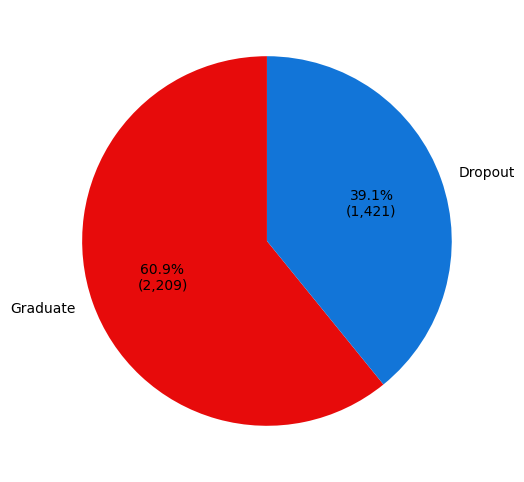
\includegraphics[width=0.70\textwidth]{images/Table_Dropout_TargetDistributionBarChart.png}
        \caption{Số lượng sinh viên theo tình trạng}
        \label{fig:Table_Dropout_TargetDistributionBarChart}
    \end{figure}

    \FloatBarrier
    
    Biểu đồ pie(\ref{graph:pie}) \ref{fig:Table_Dropout_TargetDistributionBarChart} cho thấy sự phân phối dữ liệu giữa nhãn Dropout (đã nghỉ học) và Graduate (đã tốt nghiệp). Dữ liệu 2 nhãn có phân phối gần 40:60, có mất cân bằng nhẹ. 


     \begin{figure}[htp]
        \centering
        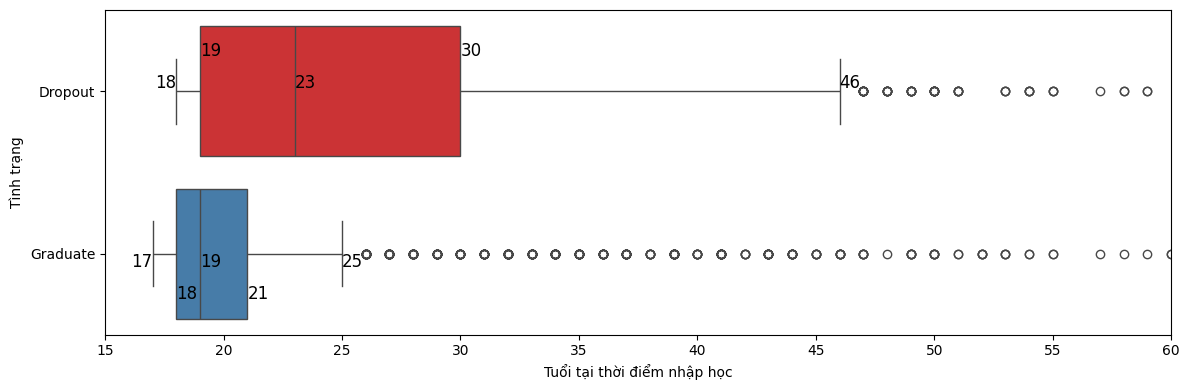
\includegraphics[width=0.95\textwidth]{images/Table_Dropout_Age_Target.png}
        \caption{Tuổi khi nhập học theo tình trạng}
        \label{fig:Table_Dropout_Age_Target}
    \end{figure}

    \FloatBarrier

    Biểu bồ boxplot(\ref{graph:boxplot}) \ref{fig:Table_Dropout_Age_Target} cho thấy tồn tại các sinh viên tốt nghiệp dù độ tuổi nhập học cao, nhưng đa phần sinh viên tốt nghiệp là người nhập học trong độ tuổi 18-21. Qua 25 tuổi nhập học mà tốt nghiệp đã có thể xem là ngoại lệ. Nhóm bỏ học cao hơn rõ ràng, cho thấy độ tuổi nhập học cao có liên hệ với nguy cơ bỏ học.

    Xét số môn tích lũy hk 1 có trường hợp ngoại lệ cao, áp dụng $UpperFence = Q_3 + 1.5 *IQR = 6 + 1.5*3 = 10.5$ (bảng \ref{tab:stat-dropout}), ta chọn số tín chỉ = 11 là tối đa để loại bỏ các điểm ngoại lệ. Từ đó xây dựng biểu đồ hình \ref{fig:Table_Dropout_Sem1Units_Dropout} và hình \ref{fig:Table_Dropout_Sem1Units_Graduate}
        
    \begin{figure}[htp]
        \centering
        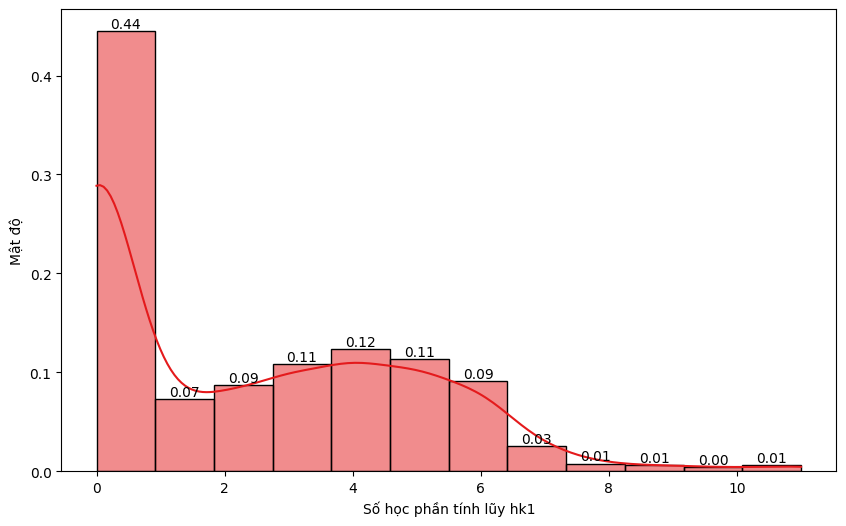
\includegraphics[width=0.95\textwidth]{images/Table_Dropout_Sem1Units_Dropout.png}
        \caption{Phân phối số môn tích lũy hk 1 nhóm Dropout}
        \label{fig:Table_Dropout_Sem1Units_Dropout}
    \end{figure}

    \FloatBarrier
    
    Biểu đồ histogram(\ref{graph:hist}) \ref{fig:Table_Dropout_Sem1Units_Dropout} thể hiện phân phối số môn tích lũy học kỳ một nhóm Dropout lệch về phải, phần lớn sinh viên bỏ học tích lũy ít học phần, số lượng tích lũy nhiều học phần giảm dần. Cột 0 học phần chiếm phân phối cao nhất ở 0.44, cho thấy sinh viên không tích lũy được học phần nào có nguy cơ bỏ học cao nhất. Đường KDE với đỉnh ở cột 0, cong giảm dần dần về bên phải cũng phản ánh điều tương tự, nhóm sinh viên bỏ học sẽ có xu hướng tích lũy được ít hoặc không môn nào.

    \begin{figure}[htp]
        \centering
        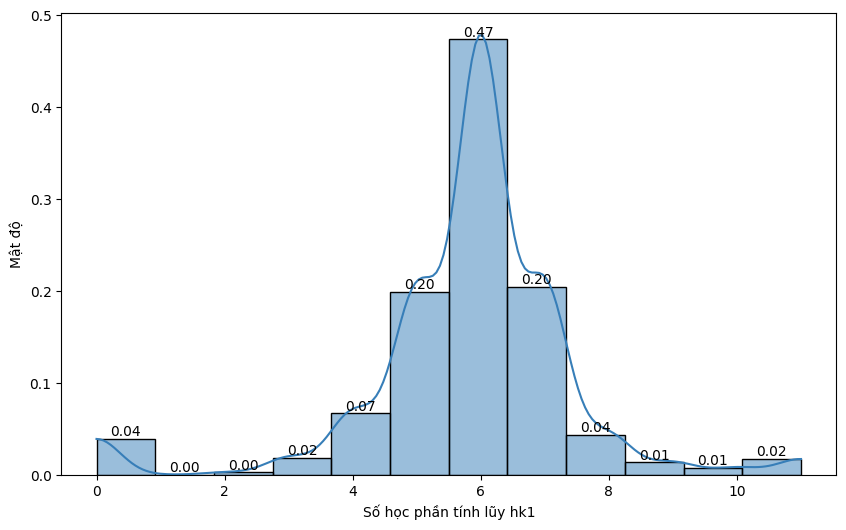
\includegraphics[width=0.95\textwidth]{images/Table_Dropout_Sem1Units_Graduate.png}
        \caption{Phân phối số môn tích lũy hk 1 nhóm Graduate}
        \label{fig:Table_Dropout_Sem1Units_Graduate}
    \end{figure}

    \FloatBarrier

     Biểu đồ histogram \ref{fig:Table_Dropout_Sem1Units_Graduate} thể hiện phân phối số môn tích lũy học kỳ một nhóm Graduate là dạng chuẩn, đỉnh phân bố tập trung tại 6 môn. Đường KDE có hình chuông, đối xứng quanh trung tâm, cho thấy phần lớn sinh viên tốt nghiệp đều đạt được mức học phần tích lũy tương đối, với một số rất ít trường hợp đặc biệt tích lũy rất ít hoặc nhiều học phần.

    Số môn tích lũy hk 2 cũng tồn tại trường hợp ngoại lệ cao, lần nữa áp dụng $UpperFence = Q_3 + 1.5 *IQR = 6 + 1.5*4 = 12$ (bảng \ref{tab:stat-dropout}), ta chọn số tín chỉ = 12 là tối đa để loại bỏ các điểm ngoại lệ. 
    
     \begin{figure}[htp]
        \centering
        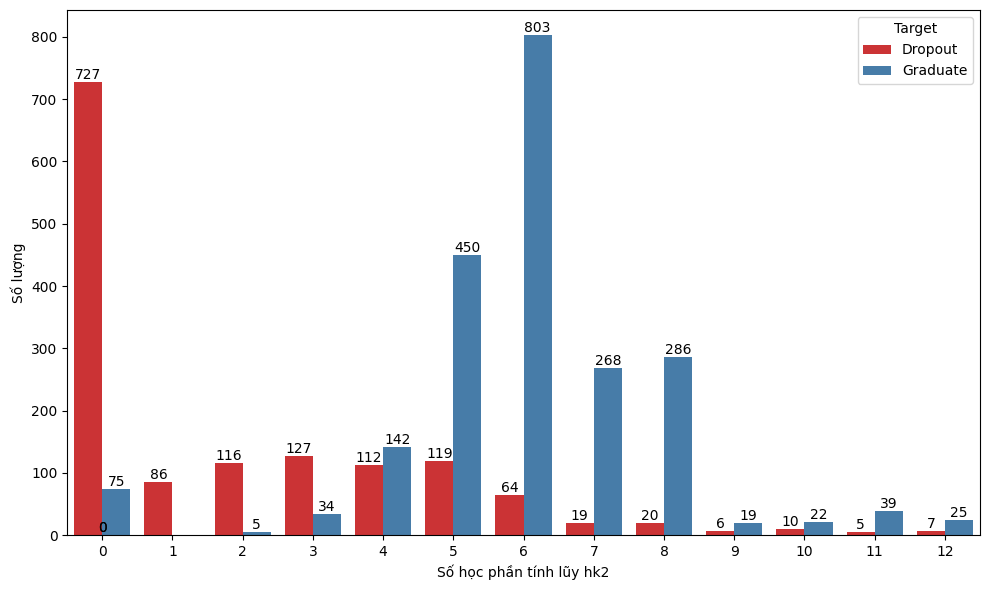
\includegraphics[width=0.95\textwidth]{images/Table_Dropout_Sem2Units.png}
        \caption{Phân phối số môn tích lũy hk 2}
        \label{fig:Table_Dropout_Sem2Units}
    \end{figure}

    \FloatBarrier

     Biểu đồ cột(\ref{graph:bar}) \ref{fig:Table_Dropout_Sem2Units} cho thấy khác biệt rõ rệt số môn tích lũy hk 2 giữa nhóm bỏ học và tốt nghiệp. Nhóm sinh viên bỏ học thường có số môn đạt được trong kỳ thấp có số lượng áp đảo, nhiều nhất ở cột 0. Ngược lại, những sinh viên tích lũy được từ 5 học phần trở lên thuộc nhóm tốt nghiệp cao hơn đáng kể, số lượng vượt xa số bỏ học. 

    Từ các biểu đồ phân tích số học phần tích lũy hai kỳ, có thể kết luận số môn đạt được mỗi kỳ liên quan chặt chẽ với tình trạng bỏ học, với sinh viên có số tích lũy ít có xu hướng bỏ học cao.

    \begin{figure}[htp]
        \centering
        \begin{subfigure}{0.45\textwidth}
            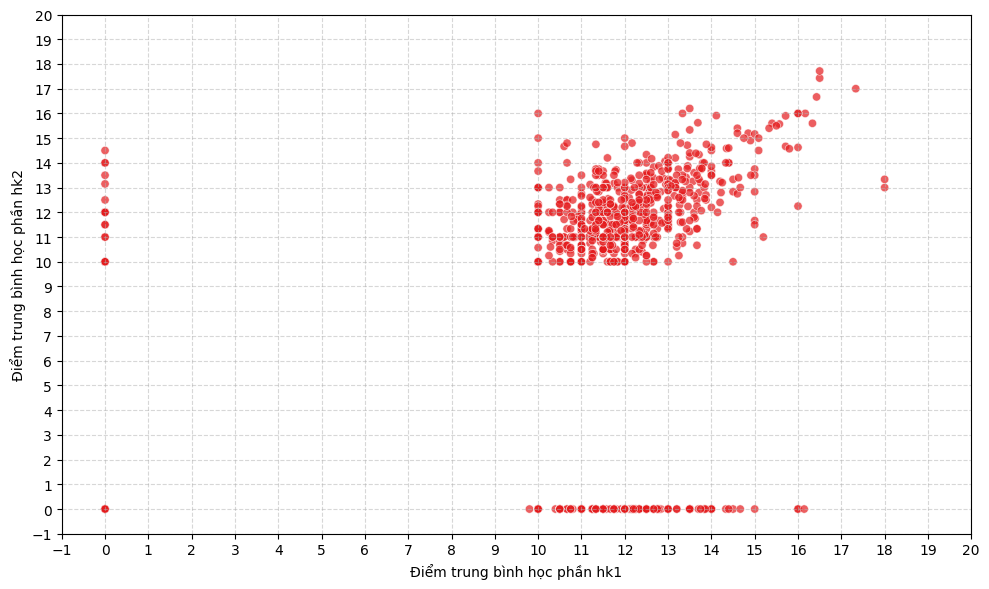
\includegraphics[width=\textwidth]{images/Table_Dropout_GradeDropout_Target.png}
            \caption{Dropout}
            \label{fig:Table_Dropout_GradeDropout_Target}
        \end{subfigure}
        \hfill
        \begin{subfigure}{0.45\textwidth}
            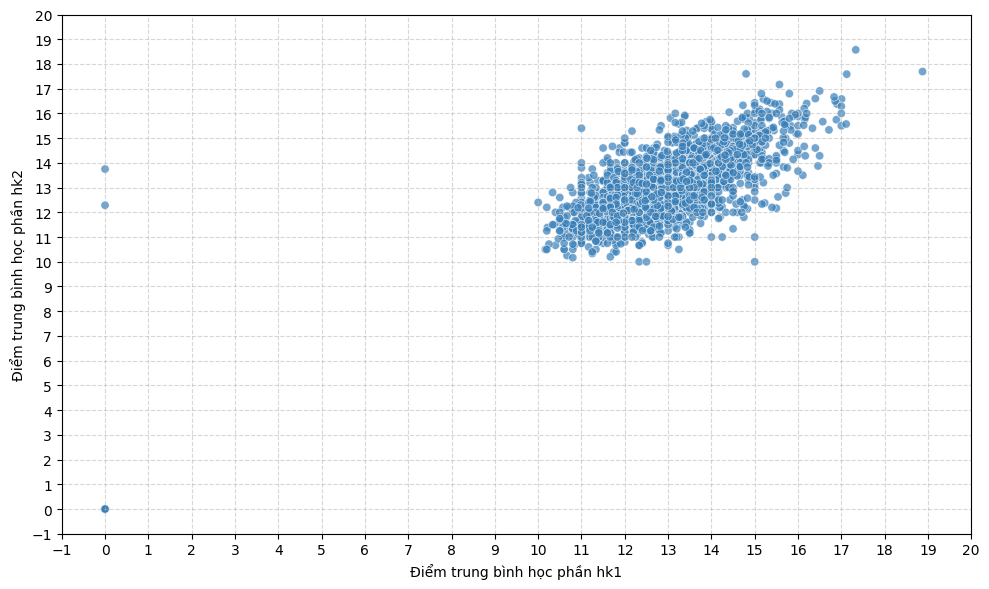
\includegraphics[width=\textwidth]{images/Table_Dropout_GradeGraduate_Target.png}
            \caption{Graduate}
            \label{fig:Table_Dropout_GradeGraduate_Target}
        \end{subfigure}
        \caption{Phân bố điểm trung bình sinh viên}
        \label{fig:Table_Dropout_GradeGraduate_Target}
    \end{figure}

    \FloatBarrier

    Các biểu đồ Scatter(\ref{graph:scatter}) \ref{fig:Table_Dropout_GradeGraduate_Target} thể hiện quan hệ điểm trung bình hk1, hk2 và tình trạng của sinh viên. Hình \ref{fig:Table_Dropout_GradeGraduate_Target} cho thấy nhóm tốt nghiệp toàn bộ (trừ một vài rất ít điểm ngoại lệ) có điểm trung bình cả hai kỳ hoàn toàn trên trung bình và tập trung ở vùng có điểm cao. Trong khi đó, từ hình \ref{fig:Table_Dropout_GradeDropout_Target} thấy được ở nhóm bỏ học, có nhiều trường hợp bỏ học/thi/rớt môn một hoặc cả hai kỳ, tạo thành các điểm trên đường x=0, y=0 và điểm (0,0). Nhiều điểm tập trung chính xác trên đường x=10 và y=10, có thể suy đoán đây là các trường hợp được vớt điểm đủ trung bình.

    Dữ liệu điểm hai học kỳ không có giá trị trong khoảng (0, 10), có thể thấy với bộ dữ liệu các trường hợp có điểm dưới trung bình, rớt môn, sẽ không được tính điểm tích lũy. Từ đó, để nhìn rõ hơn 2 cụm điểm nhóm tốt nghiệp và bỏ học, ta vẽ hình \ref{fig:Table_Dropout_GradeGraduate_Target_ZoomIn} với trục x, y giới hạn để phóng to đoạn 10-20.

    \begin{figure}[htp]
        \centering
        \begin{subfigure}{0.80\textwidth}
            \centering
            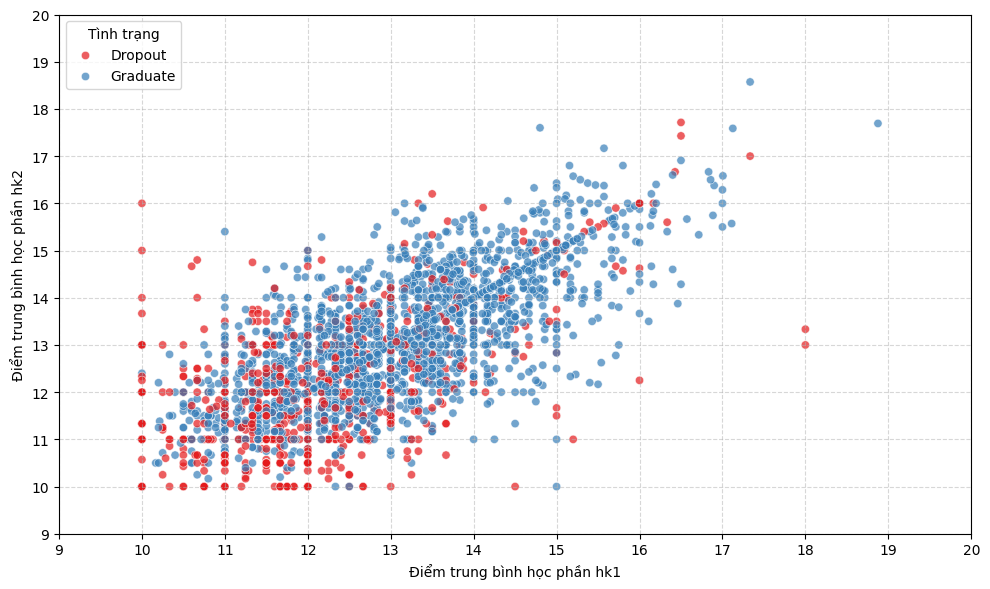
\includegraphics[width=\textwidth]{images/Table_Dropout_Grade_Target_ZoomIn.png}
            \caption{Kết hợp}
            \label{fig:Table_Dropout_Grade_Target_ZoomIn}
        \end{subfigure}
        \vspace{0.5cm}
        \begin{subfigure}{0.45\textwidth}
            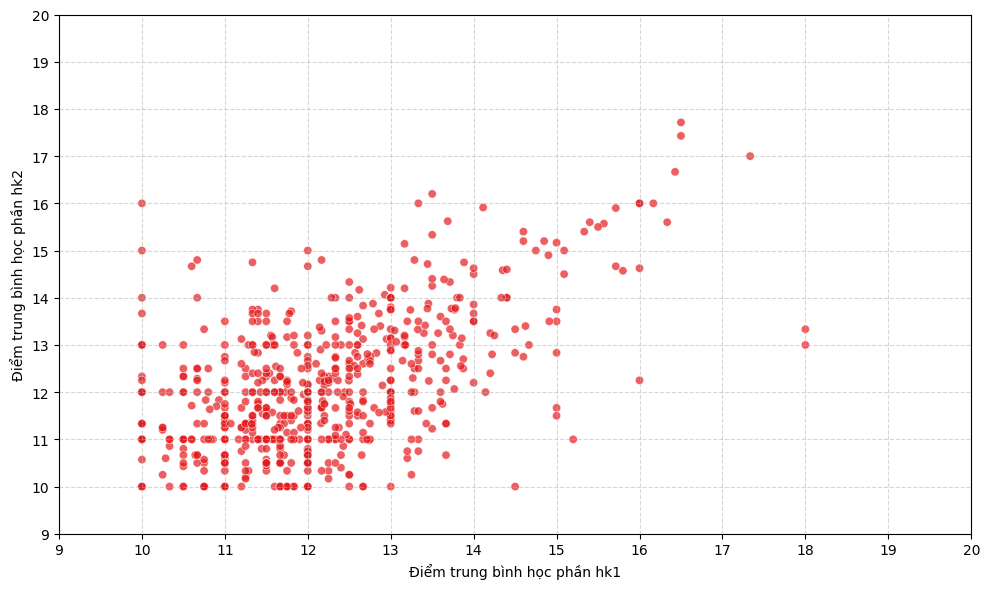
\includegraphics[width=\textwidth]{images/Table_Dropout_GradeDropout_Target_ZoomIn.png}
            \caption{Dropout}
            \label{fig:Table_Dropout_GradeDropout_Target_ZoomIn}
        \end{subfigure}
        \hfill
        \begin{subfigure}{0.45\textwidth}
            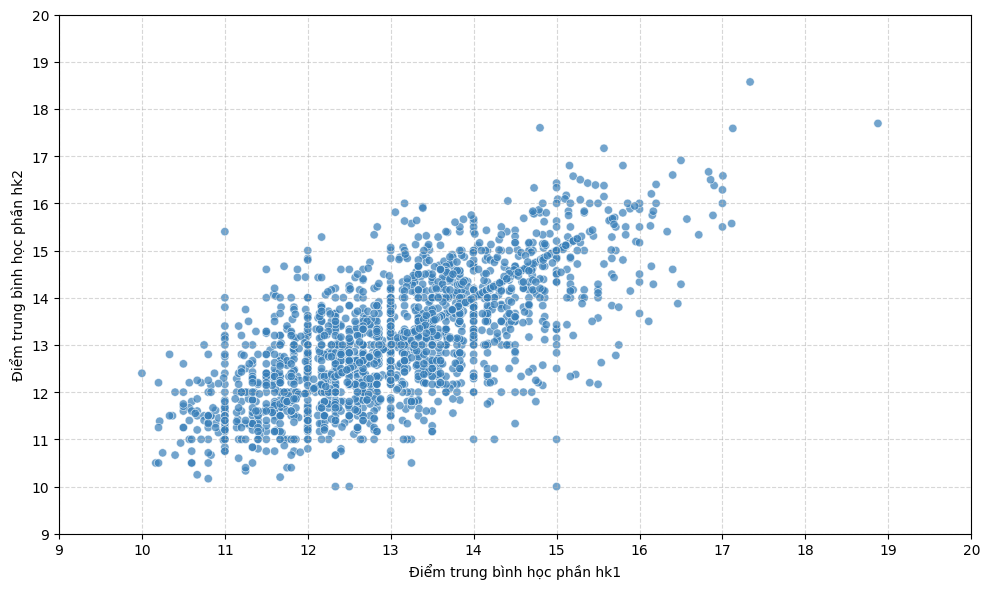
\includegraphics[width=\textwidth]{images/Table_Dropout_GradeGraduate_Target_ZoomIn.png}
            \caption{Graduate}
            \label{fig:Table_Dropout_GradeGraduate_Target_ZoomIn}
        \end{subfigure}
        \caption{Phân bố điểm trung bình sinh viên (to phóng đoạn 9-20)}
        \label{fig:Table_Dropout_GradeGraduate_Target_ZoomIn}
    \end{figure}

    \FloatBarrier

    Hình \ref{fig:Table_Dropout_GradeGraduate_Target_ZoomIn}, cho thấy rõ điểm trung bình hai kỳ nhóm tốt nghiệp cao, tạo thành một cụm từ khoảng 12-16 điểm cho cả 2 kỳ. Còn nhóm rớt môn có cụm điểm phân tán hơn, hướng về dưới và bên trái, tức điểm của hai kỳ có xu hướng nhỏ hơn so với nhóm tốt nghiệp. Từ hai hình \ref{fig:Table_Dropout_GradeGraduate_Target}, \ref{fig:Table_Dropout_GradeGraduate_Target_ZoomIn}, có thể kết luận điểm số trung bình có mối quan hệ với tình trạng bỏ học của sinh viên, đặc biệt khi điểm gần sát mức trung bình hoặc dưới trung bình (0đ).

    \begin{figure}[htp]
        \centering
        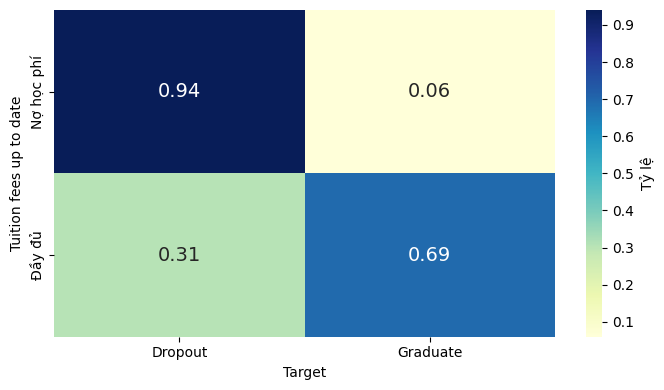
\includegraphics[width=0.95\textwidth]{images/Table_Dropout_Fee_Target.png}
        \caption{Liên hệ giữa tình trạng nợ học phí và tình trạng sinh viên}
        \label{fig:Table_Dropout_Fee_Target}
    \end{figure}

    \FloatBarrier

    Biểu đồ heatmap(\ref{graph:heatmap}) hình \ref{fig:Table_Dropout_Fee_Target} thể hiện phần lớn sinh viên bỏ học có xu hướng nợ học phí, chiếm tỉ lệ đến 0.94. Còn các sinh viên đóng học phí đầy đủ, chỉ 0.31 bỏ học. Từ đây cho thấy tình trạng nợ học phí có mối quan hệ mạnh với nguy cơ bỏ học.


\subsubsection{Data transformation}

    Biểu diễn các thuật toán data transformation: min-max scaler(\ref{scaler:minmax}), standard scaler\ref{scaler:standard}), robust scaler(\ref{scaler:robust}), Max ABS scaler(\ref{scaler:maxabs}), Quantile scaler(\ref{scaler:quantile}) trên cột 'Curricular units 1st sem (grade)' ta thu được bảng thống kê sau:

    \begin{table}[htbp]
    \centering
    \caption{ Biểu diễn thống kê cột 'Curricular units 1st sem (grade)' qua các scaler}
    \label{tab:stat-dropout-scaler}
    \begin{tabular}{|l|l|l|l|l|l|l|}
        \hline
         & Dữ liệu gốc & Min-Max & Standard & Robust & MaxAbs & Quantile \\
        \hline
        Mean & 10.535 & 0.558 & 0 & -0.723 & 0.558 & 0.484 \\
        \hline
        Min & 0 & 0 & -2.083 & -4.937 & 0 & 0 \\
        \hline
        Q1 & 11 & 0.583 & 0.092 & -0.537 & 0.583 & 0.249 \\
        \hline
        Median & 12.341 & 0.654 & 0.357 & 0 & 0.654 & 0.5 \\
        \hline
        Q3 & 13.5 & 0.715 & 0.586 & 0.463 & 0.715 & 0.754 \\
        \hline
        Max & 18.875 & 1 & 1.649 & 2.613 & 1 & 1 \\
        \hline
        Mode & 0 & 0 & -2.083 & -4.937 & 0 & 0 \\
        \hline
        Var & 25.58 & 0.072 & 1 & 4.093 & 0.072 & 0.097 \\
        \hline
        SD & 5.058 & 0.268 & 1 & 2.023 & 0.268 & 0.312 \\
        \hline
        CV & 0.48 & 0.48 &  & -2.8 & 0.48 & 0.644 \\
        \hline
        IQR & 2.5 & 0.132 & 0.494 & 1 & 0.132 & 0.505 \\
        \hline
    \end{tabular}
    \end{table}

    \FloatBarrier

    \begin{figure}[htp]
        \centering
        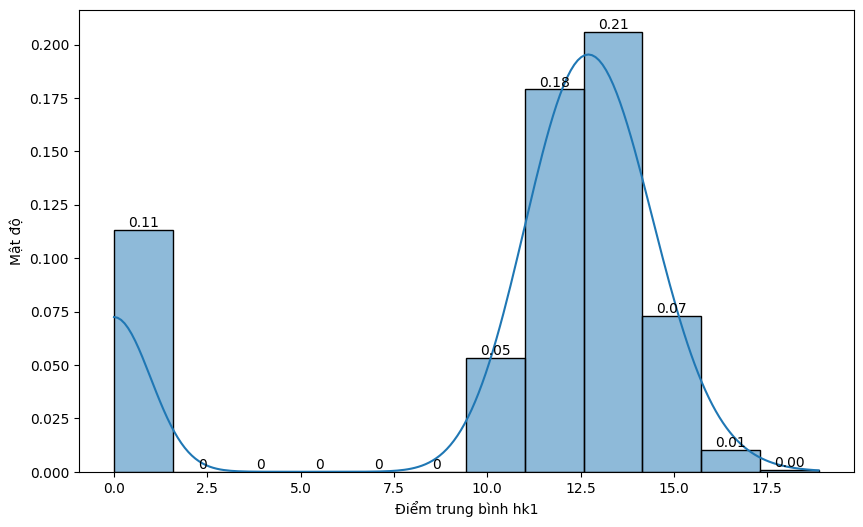
\includegraphics[width=0.80\textwidth]{images/Table_Dropout_Grade_Norm.png}
        \caption{Histogram 'Curricular units 1st sem (grade)' gốc}
        \label{fig:Table_Dropout_Grade_Norm}
    \end{figure}

    \begin{figure}[htp]
        \centering
        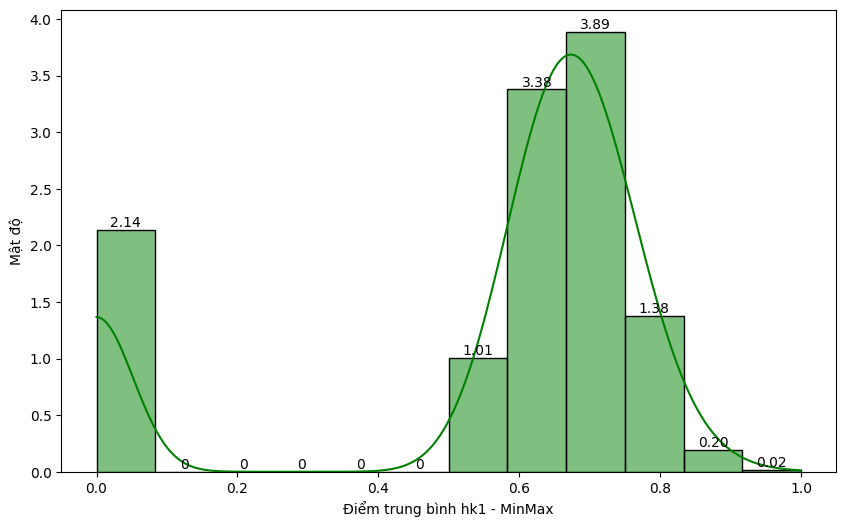
\includegraphics[width=0.80\textwidth]{images/Table_Dropout_Grade_MinMax.png}
        \caption{Histogram 'Curricular units 1st sem (grade)' qua Min-Max Scaler}
        \label{fig:Table_Dropout_Grade_MinMax}
    \end{figure}

    \FloatBarrier
    
    Min-Max scaler biến đổi dữ liệu về khoảng [0, 1]. Min, max của đặc trưng 'Curricular units 1st sem (grade)' trở thành 0, 1. Trung bình trở thành 0.558,... (bảng \ref{tab:stat-dropout-scaler}). Khoảng giá trị dữ liệu thay đổi nhưng hình dáng phân phối được giữ nguyên (hình \ref{fig:Table_Dropout_Grade_MinMax})

    \begin{figure}[htp]
        \centering
        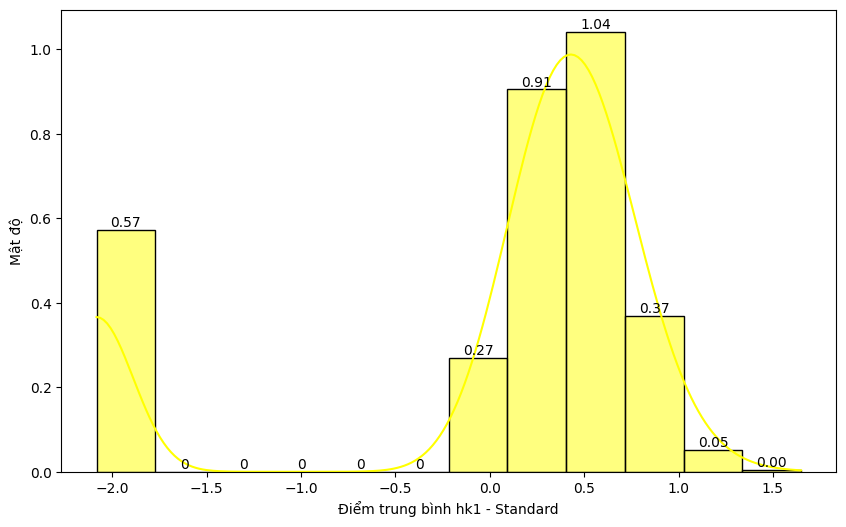
\includegraphics[width=0.80\textwidth]{images/Table_Dropout_Grade_Standard.png}
        \caption{Histogram 'Curricular units 1st sem (grade)' qua Standard Scaler}
        \label{fig:Table_Dropout_Grade_Standard}
    \end{figure}

    \FloatBarrier

    Standard scaler chuyển dữ liệu về mean = 0 và sd = 1. Dữ liệu mới có min, max = -2.083, 1.649 (bảng \ref{tab:stat-dropout-scaler}). CV không thể tính được vì mean = 0. Hình dáng dữ liệu được giữ nguyên (hình \ref{fig:Table_Dropout_Grade_Standard})

    \begin{figure}[htp]
        \centering
        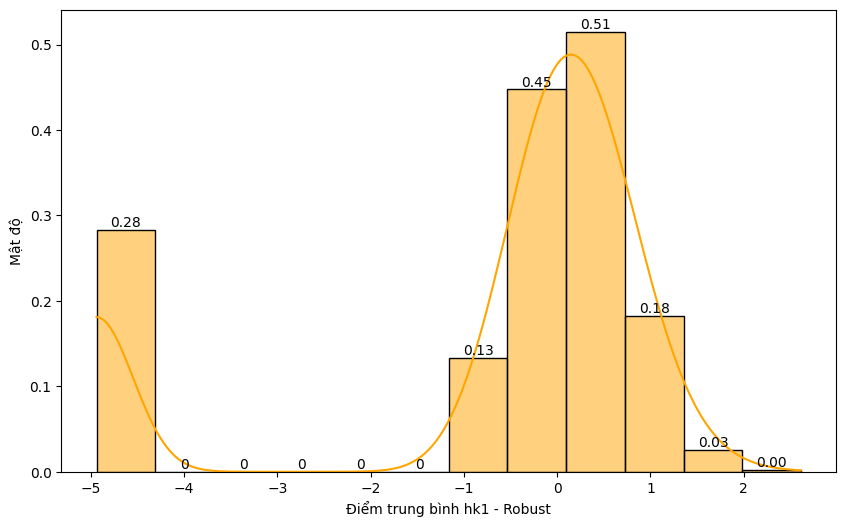
\includegraphics[width=0.80\textwidth]{images/Table_Dropout_Grade_Robust.png}
        \caption{Histogram 'Curricular units 1st sem (grade)' qua Robust Scaler}
        \label{fig:Table_Dropout_Grade_Robust}
    \end{figure}

    \FloatBarrier

    Robust scaler sử dụng trung vị thay vì trung bình và IQR thay vì độ lệch chuẩn (\ref{scaler:robust}), nên kết quả sau chuẩn hóa cho trung vị bằng 0 và IQR bằng 1, tuy nhiên các giá trị lớn và nhỏ vẫn giữ nguyên độ lệch lớn so với phần giữa: min, max có giá trị -4.937, 2.613, lớn hơn khoảng so với sử dụng standard scaler (bảng \ref{tab:stat-dropout-scaler}). Hình dáng dữ liệu được giữ nguyên (hình \ref{fig:Table_Dropout_Grade_Robust})

    \begin{figure}[htp]
        \centering
        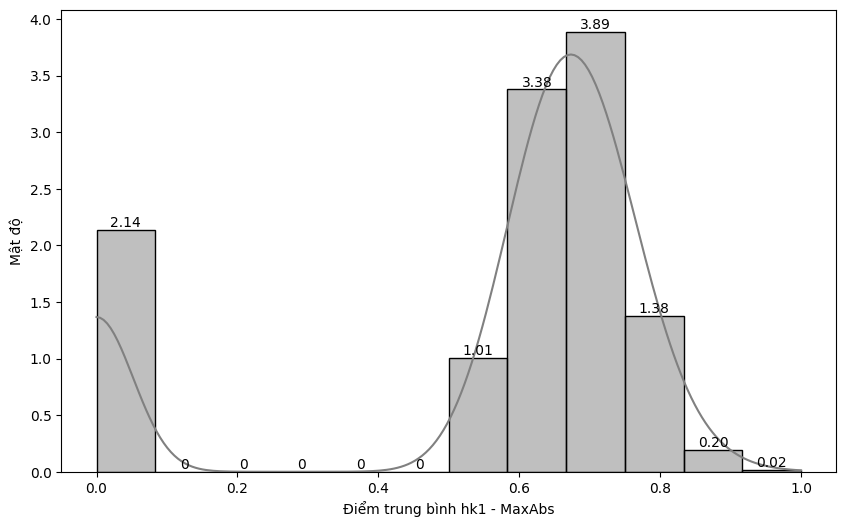
\includegraphics[width=0.80\textwidth]{images/Table_Dropout_Grade_MaxABS.png}
        \caption{Histogram 'Curricular units 1st sem (grade)' qua Max ABS Scaler}
        \label{fig:Table_Dropout_Grade_MaxABS}
    \end{figure}

    \FloatBarrier

    Max ABS scaler chia từng điểm dữ liệu cho giá trị tuyệt đối lớn nhất (\ref{scaler:maxabs}) để đưa dữ liệu về đoạn [-1, 1]. Tuy nhiên dữ liệu cột điểm trung bình hk 1 ở đây không có dữ liệu âm, nên kết quả thu được là tương tự với Min-Max Scaler (bảng \ref{tab:stat-dropout-scaler}, hình \ref{fig:Table_Dropout_Grade_MaxABS})

    

    \begin{figure}[htp]
        \centering
        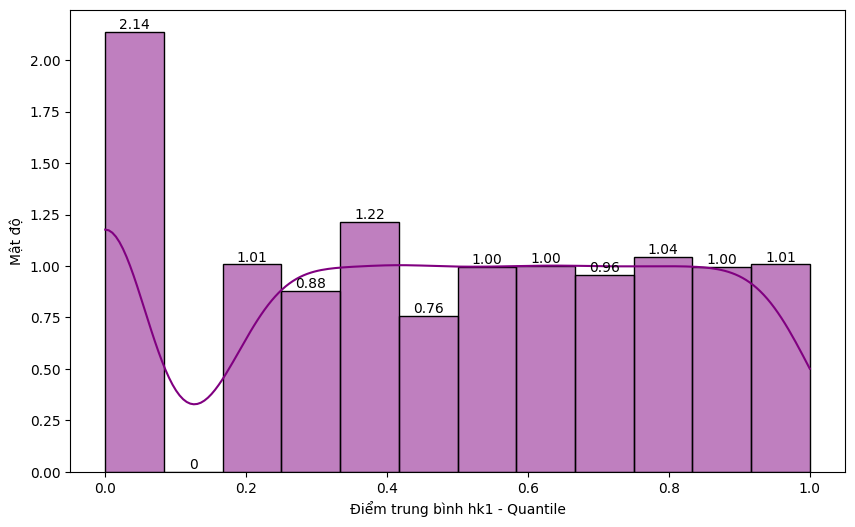
\includegraphics[width=0.80\textwidth]{images/Table_Dropout_Grade_Quantile.png}
        \caption{Histogram 'Curricular units 1st sem (grade)' qua Quantile Scaler}
        \label{fig:Table_Dropout_Grade_Quantile}
    \end{figure}

    \FloatBarrier

    Quantile Scaler chuyển dữ liệu về phân phối đều trong khoảng [0,1] (\ref{scaler:quantile}), nên hình dánh phân phối trở nên khá phẳng (hình \ref{fig:Table_Dropout_Grade_Quantile}); Q1, trung vị, Q3 trở thành gần chính xác 0.25, 0.5, 0.75 (bảng \ref{tab:stat-dropout-scaler})

\subsubsection{Mô hình hóa dữ liệu}
    \paragraph{Cấu hình cài đặt} \label{paragraph:model-setup}
    \leavevmode

    Các mô hình sử dụng:

    \begin{itemize}
        \item \textbf{Logistic Classification}: 

            \begin{lstlisting}[language=Python]
                LogisticRegressionCV(
                    max_iter=max_iter,
                    Cs=cs,
                )
            \end{lstlisting}

            khoảng hypertune tham số

            \begin{lstlisting}[language=Python]
                list_max_iter = [10, 20, 30, 40, 50, 100, 200, 300, 500]
                list_cs = [1,2,3,4,5,8,10]
            \end{lstlisting}.

        \item \textbf{Random Forest Classifier}:

            \begin{lstlisting}[language=Python]
                RandomForestClassifier(
                    max_depth=max_depth,
                    n_estimators=n_estimators,
                    min_samples_leaf=min_samples_leaf,
                )
            \end{lstlisting}

            khoảng hypertune tham số

            \begin{lstlisting}[language=Python]
                list_max_depth = [2, 3, 5, 10]
                list_n_estimators = [50, 100, 150, 200]
                list_min_samples_leaf = [3, 5, 10, 20]
            \end{lstlisting}.

        \item \textbf{XGBoost Classifier}:
            \begin{lstlisting}[language=Python]
                XGBClassifier(
                    max_depth=max_depth,
                    n_estimators=n_estimators,
                    reg_lambda=reg_lambda,
                    learning_rate=lr,
                )
            \end{lstlisting}

            khoảng hypertune tham số

            \begin{lstlisting}[language=Python]
                list_max_depth = [2, 3, 4, 5]
                list_lambda = [3, 2, 1, 0.5]
                list_learning_rate = [0.5, 0.25, 0.1, 0.05]
                list_n_estimators = [25, 50, 100, 150]
            \end{lstlisting}.
        
    \end{itemize}

    Thuật toán data transform sử dụng: Do dữ liệu có nhiều điểm ngoại lệ, nhóm chọn Robust Scaler để chuẩn hóa dữ liệu.

    Chia tập dữ liệu huấn luyện: Cross-validation 5 folds.

    \paragraph{Phân lớp tình trạng sinh viên}
    \leavevmode

    Chọn các đặc trưng huấn luyện: 'Tuition fees up to date',
    'Scholarship holder',
    'Debtor', 'Application order', 
    'Age at enrollment', 
    'Curricular units 1st sem (approved)', 
    'Curricular units 1st sem (grade)',
    'Curricular units 2nd sem (approved)', 
    'Curricular units 2nd sem (grade)'


    Kết quả:
    \begin{itemize}
        \item \textbf{Logistic Classification}: 
        
            Mô hình tốt nhất:
            \begin{itemize}
                \item max\_iter: 10
                \item cs: 2
            \end{itemize}

            \begin{table}[htbp]
            \centering
            \caption{Kết quả Logistic Classification - Phân lớp tình trạng sinh viên}
            \label{tab:LogCV-Dropout}
            \begin{tabular}{lrrrrrr}
                \hline
                & train\_acc & test\_acc & test\_recall & test\_precision & test\_f1 & test\_roc\_auc \\
                \hline
                mean & 0.889935 & 0.889082 & 0.818310 & 0.894695 & 0.854619 & 0.930804 \\
                std & 0.001182 & 0.005009 & 0.019150 & 0.010877 & 0.007953 & 0.008678 \\
                min & 0.888097 & 0.881766 & 0.803571 & 0.881481 & 0.844278 & 0.921640 \\
                max & 0.891266 & 0.894437 & 0.850000 & 0.908000 & 0.865455 & 0.942839 \\
                \hline
            \end{tabular}
            \end{table}
  
            
            \FloatBarrier

        \item \textbf{Random Forest Classifier}:

            Mô hình tốt nhất:
            \begin{itemize}
                \item max\_depth: 10
                \item n\_estimators: 100
                \item min\_samples\_leaf: 3
            \end{itemize}

            \begin{table}[htbp]
                \centering
                \caption{Kết quả Random Forest Classifier - Phân lớp tình trạng sinh viên}
                \label{tab:RF-Dropout}
                \begin{tabular}{lrrrrrr}
                    \hline
                     & train\_acc & test\_acc & test\_recall & test\_precision & test\_f1 & test\_roc\_auc \\
                    \hline
                    mean & 0.921657 & 0.895071 & 0.824762 & 0.903870 & 0.862393 & 0.940038 \\
                    std & 0.002541 & 0.008536 & 0.014551 & 0.016729 & 0.011015 & 0.006931 \\
                    min & 0.918746 & 0.886040 & 0.800000 & 0.888889 & 0.848485 & 0.933446 \\
                    max & 0.925517 & 0.907275 & 0.838710 & 0.931452 & 0.876660 & 0.951630 \\
                    \hline
                \end{tabular}
            \end{table}
            
            \FloatBarrier

        \item \textbf{XGBoost Classifier}:
        
            Mô hình tốt nhất:
            \begin{itemize}
                \item max\_depth: 4
                \item n\_estimators: 100
                \item reg\_lambda: 3
                \item learning\_rate: 0.1
            \end{itemize}

            \begin{table}[htbp]
                \centering
                \caption{Kết quả XGBoost Classifier - Phân lớp tình trạng sinh viên}
                \label{tab:XGB-Dropout}
                \begin{tabular}{lrrrrrr}
                \hline
                 & train\_acc & test\_acc & test\_recall & test\_precision & test\_f1 & test\_roc\_auc \\
                \hline
                mean & 0.917023 & 0.895355 & 0.823323 & 0.905815 & 0.862492 & 0.937652 \\
                std & 0.003497 & 0.009013 & 0.016033 & 0.015954 & 0.011883 & 0.006926 \\
                min & 0.913400 & 0.883191 & 0.796429 & 0.885496 & 0.844697 & 0.928940 \\
                max & 0.921953 & 0.904422 & 0.839286 & 0.924000 & 0.873346 & 0.947808 \\
                \hline
                \end{tabular}
            \end{table}

            \FloatBarrier
    \end{itemize}

    So sách các mô hình:

    \begin{table}[htbp]
        \centering
        \caption{So sánh kết quả các mô hình - Dự đoán tình trạng sinh viên}
        \label{tab:compare-dropout}
        \begin{tabular}{|p{2cm}|p{2cm}|p{2cm}|p{2cm}|p{2cm}|p{2cm}|}
            \hline
             Model & Mean Test Accuracy & Mean F1 & Mean Recall & Mean Precision & Mean ROC AUC \\
            \hline
            Logistic Regression & 0.889082 & 0.854619 & 0.818310 & 0.894695 & 0.930804 \\
             \hline
             Random Forest & 0.895071 & 0.862393 & \textbf{0.824762} & 0.903870 & \textbf{0.940038} \\
             \hline
            XGBoost & \textbf{0.895355} & \textbf{0.862492} & 0.823323 & \textbf{0.905815} & 0.937652 \\
            \hline
        \end{tabular}
    \end{table}

    \FloatBarrier

    XGBoost, là mô hình phức tạp nhất, cho kết quả tốt nhất, dẫn đầu ở Accuracy, F1 và Precision. Random Forest có riêng Recall và ROC AUC cao hơn, nếu phát hiện sinh viên bỏ học (recall cao) được xem qua quan trọng hơn kết quả toàn diện thì có thể ưu tiên mô hình Random Forest.

\subsubsection{Kết luận}
    Trong phần này, nhóm đã tiến hành phân tích và xây dựng mô hình dự đoán tình trạng sinh viên. Qua mô hình hóa cho thấy các đặc trưng liên quan đến kết quả học tập các học kì đầu, tuổi nhập học và tình trạng tài chính có ảnh hưởng rõ rệt đến khả năng sinh viên bỏ học. Kết quả thu được mô hình tốt nhất XGBoost Classifier với độ chính xác 0.895, F1 0.862, Recall 0.823, Precision 0.905. Đây là cơ sở quan trọng để các cơ sở giáo dục đại học có thể sớm nhận diện và hỗ trợ các sinh viên có nguy cơ bỏ học, từ đó nâng cao hiệu quả đào tạo và giảm thiểu tỷ lệ bỏ học.